\section{Readout Matrix Unfolding}
Current and near-term quantum computing devices are subject to significant inaccuracies due to the multitudes of noise sources affecting the computation and the measurement process. With appropriate error mitigation, however, these noisy intermediate-scale quantum (NISQ) devices can still be utilized. Readout matrix unfolding is such an error mitigation protocol that combats readout errors. The protocol consists of a calibration and an unfolding sequence. Here we are considering an $n$ qubit device. The calibration is measuring the readout matrix $P$ that quantifies the measurement errors. The element $P_{ab}$ is the probability that the bitstring $b$ is measured after preparing the bitstring $a$. The matrix thus has $2^n\times2^n$ entries. For small errors rates we approximate the relation between a measured arbitrary bitstring $v'$ and the error-free bitstring $v$ as
\begin{equation}
    v_a' = \sum_b P_{ab}v_b .
    \label{eq:readout_matrix}
\end{equation}
The error mitigated result $v$ is obtained by inverting the readout matrix $P$ from the calibration and applying it to the measured bitstring $v'$. If the measurement is normalized before this procedure, then the mitigated result is still normalized and thus physical in that aspect. This is shown by looking at the absolute value of the sum over $a$ in equation \eqref{eq:readout_matrix}. The probabilistic definition of $P$ demands that all possible outcomes, here the columns, sum to unity, $\sum_a P_{ab} = 1$.
\subsubsection{Exercise 1}
\begin{equation}
        \abs{\sum_a v_a'} = \abs{\sum_{a,b}P_{ab}v_b} = \abs{\sum_b v_b} = 1
\end{equation}
While normalization is therefore guaranteed for an appropriate input, the final result $v$ might still be nonphysical, as negative entries are possible. For this report this method with an additional check against negatives values will be sufficient.
\section{Quantum Teleportation}
Quantum teleportation is a protocol to copy a quantum state $\ket{\varphi}$ over any distance between 2 locations. The sender and receiver need to share an entangled EPR qubit pair and the original state is destroyed in the process. The protocol involves preparing and measuring qubits in the EPR basis, seen in equation \eqref{eq:epr}.
\begin{equation}
    \ket{\Phi^\pm} = \frac{1}{\sqrt{2}}\left(\ket{00} \pm \ket{11}\right) \quad
    \ket{\Psi^\pm}  = \frac{1}{\sqrt{2}}\left(\ket{01} \pm \ket{10}\right)
    \label{eq:epr}
\end{equation}
\subsubsection{Exercise 2}
The preparation starting from the ground state $\ket{00}$ is achieved by creating a superposition with the Hadamard gate H and then entangling them with the CNOT gate. Figure \ref{fig:prepare_EPR} shows the circuits to create each EPR state.
\begin{figure}[h]
    \centering
    \begin{subfigure}[t]{0.19\textwidth}
        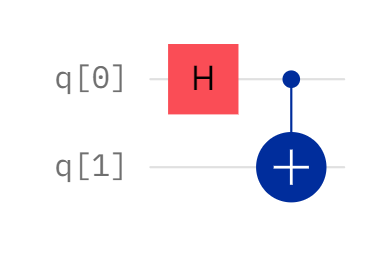
\includegraphics[width=\textwidth]{tex/figures/exercise02_01.png}
        \caption{$\ket{\Phi^+} = \frac{1}{\sqrt{2}}(\ket{00} + \ket{11}$}
        \label{fig:e0201}
    \end{subfigure}
    \begin{subfigure}[t]{0.24\textwidth}
        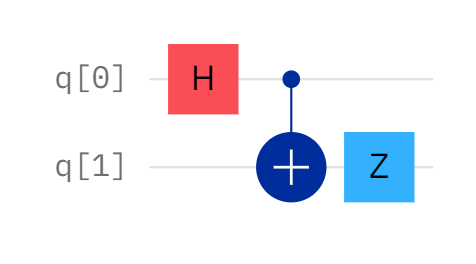
\includegraphics[width=\textwidth]{tex/figures/exercise02_02.png}
        \caption{$\ket{\Phi^-} = \frac{1}{\sqrt{2}}(\ket{00} - \ket{11}$}
        \label{fig:e0202}
    \end{subfigure}
    \begin{subfigure}[t]{0.24\textwidth}
        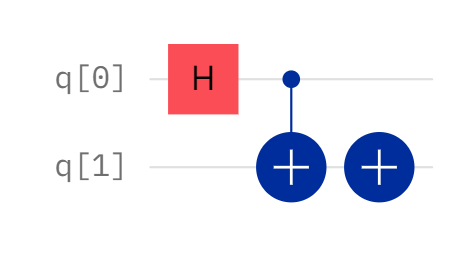
\includegraphics[width=\textwidth]{tex/figures/exercise02_03.png}
        \caption{$\ket{\Psi^+} = \frac{1}{\sqrt{2}}(\ket{01} + \ket{10}$}
        \label{fig:e0203}
    \end{subfigure}
    \begin{subfigure}[t]{0.29\textwidth}
        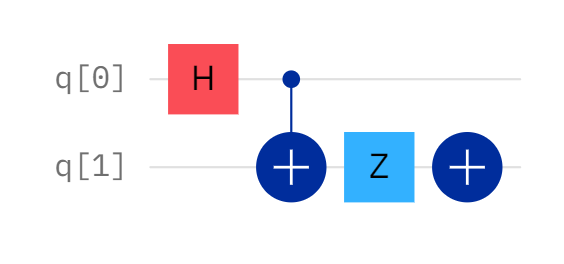
\includegraphics[width=\textwidth]{tex/figures/exercise02_04.png}
        \caption{$\ket{\Psi^-} = \frac{1}{\sqrt{2}}(\ket{01} - \ket{10}$}
        \label{fig:e0204}
    \end{subfigure}
    \caption{Preparation circuit for all EPR states. The plus symbol denotes addition modulo 2 and therefore an X or NOT gate.}
    \label{fig:prepare_EPR}
    \addtocounter{figure}{-1}
\end{figure}
To measure in the EPR basis, the gate to create $\ket{\Phi^+}$ is applied in reverse before the qubits are measured sequentially in the computational basis. The mapping between the computational basis and the EPR basis is determined by the circuit. With circuit \ref{fig:e0201} the mapping is $\ket{\Phi^+} \leftrightarrow \ket{00}$, $\ket{\Phi^-} \leftrightarrow \ket{10}$, $\ket{\Psi^+} \leftrightarrow \ket{01}$ and $\ket{\Psi^-} \leftrightarrow \ket{11}$.
\subsubsection{Exercise 3}
Depending on the outcome of the EPR measurement, a controlled unitary needs to be applied to obtain the exact original state. This is clear when the complete system state, including the original state $\ket{\varphi} = \alpha\ket{0} + \beta\ket{1}$, is rewritten in the EPR basis
\begin{equation}
\begin{aligned}
    \label{eq:decomposition}
    \ket{\varphi}_0\frac{1}{\sqrt{2}}\left(\ket{00}_{12} + \ket{11}_{12}\right) &= \ket{\Phi^+}_{01}\left(\alpha\ket{0}_2 + \beta\ket{1}_2\right) + \ket{\Phi^-}_{01}\left(\alpha\ket{0}_2 - \beta\ket{1}_2\right) \\
    &+ \ket{\Psi^+}_{01}\left(\alpha\ket{1}_2 + \beta\ket{0}_2\right)
    + \ket{\Psi^-}_{01}\left(\alpha\ket{1}_2 - \beta\ket{0}_2\right).
\end{aligned}
\end{equation}
The state of qubit q[2] after the EPR measurement will carry the $\alpha$ and $\beta$ coefficients of the original q[0] state, however, sometimes swapped or with an additional sign. The sign is removed with a controlled Z gate (CZ), the switch reversed with a controlled X gate (CX).
\begin{figure}
    \centering
    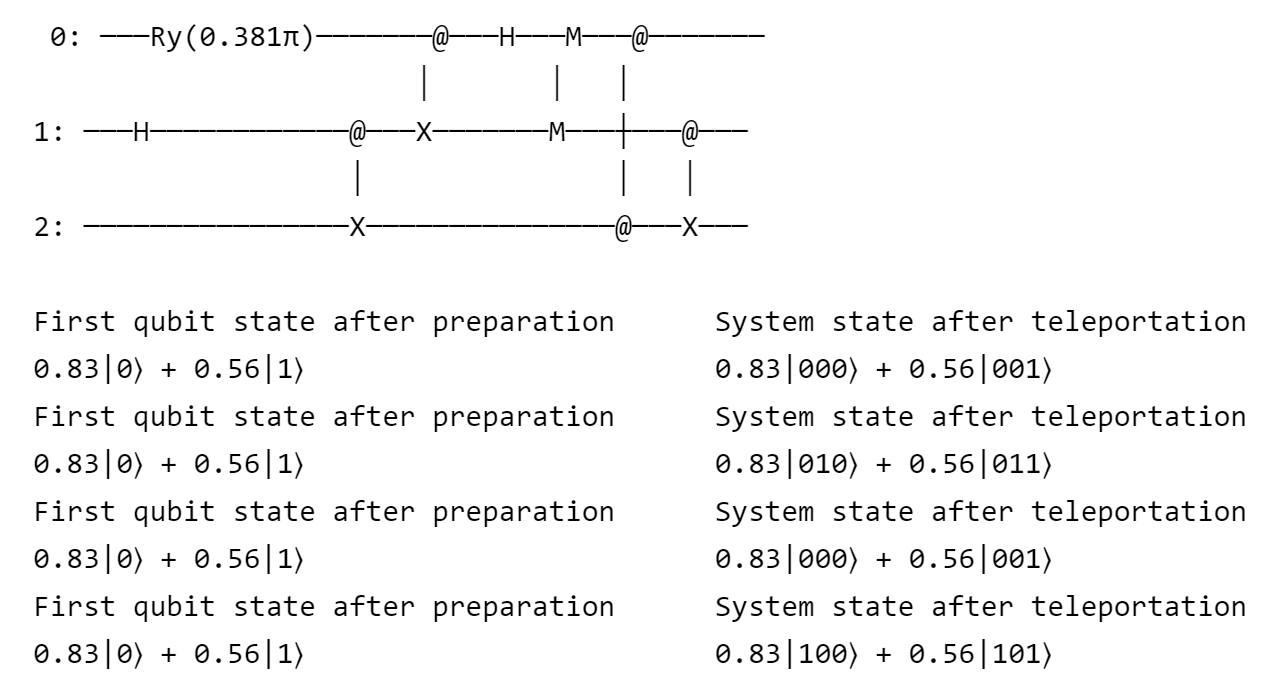
\includegraphics[width=0.8\linewidth]{tex/figures/exercise04.png}
    \caption{Circuit diagram and output for quantum teleportation. The state $\ket{\varphi}$ is initially on qubit 0 and is then copied to qubit 2. The @ symbol denotes the control qubit in a controlled gate. M shows measurements on qubits. The log shows the original and teleported state for four trials.}
    \label{fig:teleportation}
\end{figure}

\subsubsection{Exercise 4}
The complete quantum teleportation protocol is implemented and tested in the Google Cirq framework with the circuit seen in diagram \ref{fig:teleportation}. The corresponding code for all the exercises of Day 1 are found in the appendix chapter \ref{app:day1}, here we will focus on the discussion of the results. The original state $\ket{\varphi}$ is created by rotating around the y axis with a random angle, the example above uses $0.381\pi$. The log included in \ref{fig:teleportation} shows the $\alpha$ and $\beta$ values of $\ket{\varphi}$ after the rotation and the complete system state after teleportation for 4 different trials. The circuit is working correctly as qubit 2 has matching $\alpha$ and $\beta$ values in all trials, independent of the measurement results on qubit 0 and 1. In trial one and three the EPR measurement yielded $\ket{\Phi^+}$, in trial two the $\ket{\Phi^-}$ and in trial three the $\ket{\Psi^+}$ state.

\section{Rabi Oscillation}
Rabi osciallation is the primary phenomena to manipulate single qubits to any desired state. For a two-level system (TLS) quantified along the $\sigmaz$ axis, an oscillating $\sigmax$ component in the Hamiltonian
\begin{equation}
    H = -\frac{\omega_0}{2}\sigmaz + \omega_1\cos(\omega t)\sigmax
\end{equation}
will result in the system oscillating between the ground and excited state $\ket{0}$ and $\ket{1}$.  With the initial state $\ket{\Psi} = \alpha (t)\ket{0} + \beta (t)\ket{1} = \ket{0}$ the dynamics in the rotating wave approximation (RWA) are given by
\begin{equation}
\begin{aligned}
    \label{eq:dynamics}
    \alpha (t) &= e^{-i\omega t/2}\left(\cos \left(\frac{\Omega t}{2}\right) - \frac{i\Delta}{\Omega}\sin \left(\frac{\Omega t}{2}\right)\right), \\
    \beta (t) &= e^{i\omega t/2}\left(-\frac{i\omega_1}{\Omega}\sin \left(\frac{\Omega t}{2}\right)\right)
\end{aligned}
\end{equation}
where $\Delta = \omega - \omega_1$ is the detuning and $\Omega = \sqrt{\omega^2_1 + \Delta^2}$ the Rabi frequency. The condition for RWA to work well is a comparatively weak drive and a small detuning.
\begin{equation}
    \label{eq:conditions}
    \omega_1 \ll \omega_0 \quad \mathrm{and} \quad \Delta \ll 2\omega_0.
\end{equation}
\subsubsection{Exercise 5}
The population of the groud and excited states are retrieved from equations \eqref{eq:dynamics} by taking the square of the absolute value.
\begin{align}
    p_0 &= \abs{\alpha(t)}^2 = \cos^2 \frac{\Omega}{2}t + \left(\frac{\delta}{\Omega}\right)^2\sin^2\frac{\Omega t}{2}
    \label{eq:population0}
\end{align}
\begin{align}
    p_1 &= \abs{\beta (t)}^2  = \left(\frac{\omega_1}{\Omega}\right)^2\sin^2\frac{\Omega t}{2} = \left(\frac{\omega_1}{\Omega}\right)^2\frac{1}{2}\left(1-\cos\Omega t\right)
    \label{eq:population1}
\end{align}
A common method to simulate the dynamics of quantum system with a known Hamiltonian is trotterization. The relevant time interval is discretized into sufficiently small steps and the precise time evolution $U(t)$ is approximated by repeatedly applying a gate that replaces the dynamics for one time step
\begin{equation}
    U(t) = \exp\left(-i\int_0^tH(t)dt\right) \approx \prod^{N-1}_{n=0}\exp\left(-iH(n\delta t)\delta(t)\right).
    \label{eq:trotterization}
\end{equation}
\subsubsection{Exercise 6}
To test the performance of this approximation we simulate Rabi oscillations using trotterization and compare the final state with the analytical values from equation \eqref{eq:population1}. For plot \ref{fig:exercise06_01} and \ref{fig:exercise06_02} the qubit frequency is set to $\omega_0 = 25$, the driving frequency to $\omega_1 = 25.5$ with a driving strength $\omega = 2$. The frequencies are given without units as this is how they are used in the code. What is relevant for their physical properties are their values relative to each other and the considered time range. Qubit and drive are almost in resonance here with only a slight detuning $\Delta = 0.5$, meaning the Rabi frequency $\Omega = 2.062$ is very close to the driving frequency $\omega_1$ and the amplitude $\left(\frac{\omega_1}{\Omega}\right)^2$ is close to 1. This is validated by the plot \ref{fig:exercise06_01} which shows the population of the excited state undergoing a full Rabi oscillation at close to maximum amplitude. The population over the detuning seen in \ref{fig:exercise06_02} also confirms the correct timing for the simulation. At the fixed time $t = \frac{\pi}{\omega_1}$ the interaction equals a $\pi$-pulse that excites the TLS if the detuning $\Delta$ is close to zero, which is clearly visible in the plot.
\begin{figure}[h]
    \centering
    \caption{Comparison between analytical and trotterized calculations of population $\abs{\beta}^2$ for a driven two-level system. The time step for trotterization is $\delta t = 0.05$.}
    \label{fig:exercise06}
    \addtocounter{figure}{-1}
    \begin{subfigure}[t]{0.48\textwidth}
        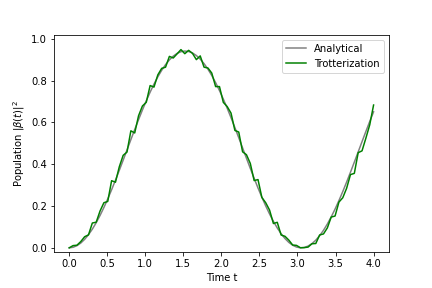
\includegraphics[width=\textwidth]{tex/figures/exercise06_01.png}
        \caption{Population $\abs{\beta}^2$ over time $t$. Rabi oscillation is clearly visible and trotterization works well. Parameters are $\omega_0 = 25, \omega_1 = 25.5$ and $\omega = 2$, resulting in the oscillation period $T = 3.047$.}
        \label{fig:exercise06_01}
    \end{subfigure}
    \begin{subfigure}[t]{0.48\textwidth}
        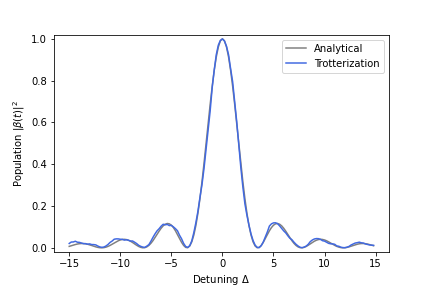
\includegraphics[width=\textwidth]{tex/figures/exercise06_02.png}
        \caption{Population $\abs{\beta}^2$ over detuning $\Delta$ at fixed time $t = \frac{\pi}{\omega_1}$. Parameters are $\omega_0 = 25, \omega_1 = 25.5$ and $\omega \in [10, 40]$ with stepsize $\delta\omega = 0.2$. The $\pi$ pulse fully excites the qubit on resonance.}
        \label{fig:exercise06_02}
    \end{subfigure}
    \\
    \begin{subfigure}[t]{0.48\textwidth}
        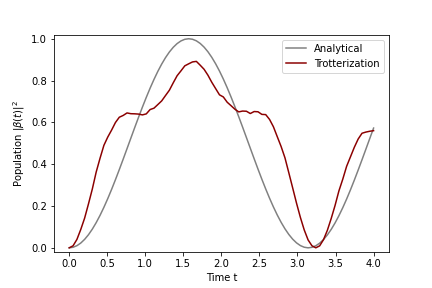
\includegraphics[width=\textwidth]{tex/figures/exercise06_03.png}
        \caption{Population $\abs{\beta}^2$ over time $t$ with $\omega_0 = \omega_1 = \omega = 2$. The driving strength is comparable to the qubit frequency, violating the conditions of the RWA. Trotterization results are more accurate here.}
        \label{fig:exercise06_03}
    \end{subfigure}
    \begin{subfigure}[t]{0.48\textwidth}
        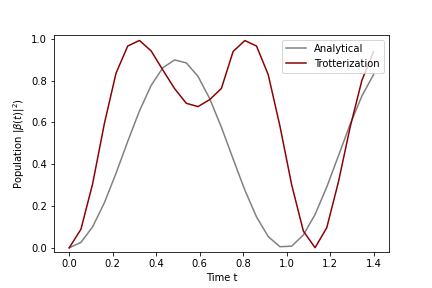
\includegraphics[width=\textwidth]{tex/figures/exercise06_04.png}
        \caption{Population $\abs{\beta}^2$ over time $t$ with $\omega_0, \omega_1, \omega = 3, 1, 6$. Calculations are not in agreement. The detuning and driving strength are larger than qubit frequency, violating all conditions of the RWA.}
        \label{fig:exercise06_04}
    \end{subfigure}
\end{figure}
\\
For the population plots seen in \ref{fig:exercise06_03} and \ref{fig:exercise06_04} the frequencies have been adjusted to $\omega_0 = \omega_1 = \omega$ and $\omega_0 = 3, \omega_1 = 1, \omega = 6$ respectively. In both cases the trotterization and analytical results yield signficantly different results. The discrepancy is explained by the applicability of the RWA used to derive the analytical equations. The driving strength $\omega_1 = 2$ in scenario \ref{fig:exercise06_03} is comparable in size to the TLS frequency $\omega_0 \sim \omega_1$. The system is therefore not in a weak driving regime and RWA is not a good solution. In scenario \ref{fig:exercise06_04} the detuning $\Delta = 3$ has been increased to be close to the TLS frequency $\Delta \sim \omega_0$. Here the parameters violate both conditions for RWA \eqref{eq:conditions} and magnify the difference between the computations.
\subsubsection{Exercise 7}
To get closer to the behavior of physical quantum devices, we extend the simulator with a noise model. These models add the decoherence effects from a physical environment of a quantum computer without simulating the environment itself. We are implementing the generalized amplitude damping channel (GAD) that describes spontaneous emission and thermal excitations. The Kraus operators of the channel are
\begin{align*}
    E_0 &= \sqrt{p}
    \begin{pmatrix}
        1 & 0 \\
        0 & \sqrt{1 - \gamma}
    \end{pmatrix}
    , \quad E_1 = \sqrt{p}
    \begin{pmatrix}
        0 & \sqrt{\gamma} \\
        0 & 0
    \end{pmatrix}
    \\ E_2 & = \sqrt{1-p}
    \begin{pmatrix}
        \sqrt{1-\gamma} & 0 \\
        0 & 1
    \end{pmatrix}
    , \quad E_3 = \sqrt{1-p}
    \begin{pmatrix}
        0 & 0 \\
        \sqrt{\gamma} & 0
    \end{pmatrix}
\end{align*}
with $1-p$ being the probability for thermal excitation and $\gamma$ the probability for spontaneous emission. The channel $\Lambda$ is then with standard definition
\begin{equation}
    \Lambda(\rho) = \sum^3_{i=0} E_i \rho E^\dagger_i .
\end{equation}
\begin{figure}[h]
    \centering
    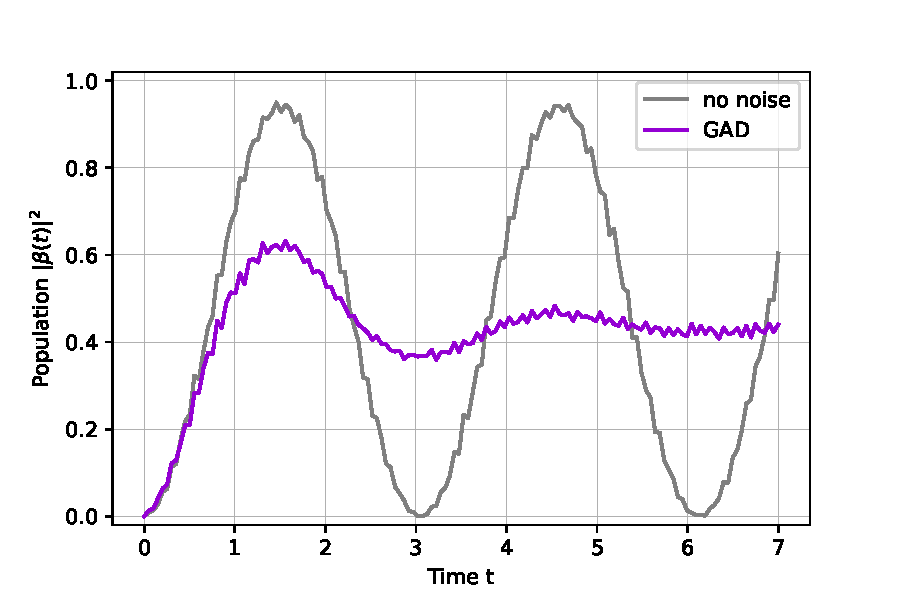
\includegraphics[width=0.7\linewidth]{tex/figures/exercise07_01.pdf}
    \caption{Comparison between trotterization with and without noise. The addition of the dampening channel clearly reduces the amplitude of the Rabi oscillation. Parameters for the system, noise model and trotterization are $\omega_0 = 25.5, \omega_1 = 25, \omega = 2$, $p = 0.9, \gamma = 0.02$ and $\delta t = 0.05$.}
    \label{fig:exercise07_01}
\end{figure}
The diagram \ref{fig:exercise07_01} shows a direct comparison between the simulation with and without the GAD. The introduction of decoherence results in a dampened oscillation that approaches a stable population. The strength of the dampening is determined by $\gamma$, which is clearly visible in \ref{fig:exercise07_03}. The oscillation with $\gamma = 0.02$ fades out within the simulation time, while the population for $\gamma = 0.005$ oscillates even beyond the visible interval. The peaks of the Rabi oscillation fall exponentially, characterized by the $T_1$ decoherence time. The second dominating feature in the graphs is the asymptote, which is controlled by the thermal excitation probability $p$ and the Rabi drive. This is demonstrated in \ref{fig:exercise07_02} where the lower value for $p$, corresponding to higher thermal excitation rates, concludes in a higher limit after oscillation. Even between the edge cases $p = 0$ and 1 shown in \ref{fig:exercise07_02}, the difference in the final limit is fairly small considering the available range is $[0, 1]$. This is due to the Rabi oscillations driving the TLS to a population around the median $0.5$ and away from the extreme cases $\alpha = 1$ or $\beta = 1$. The progression without any Rabi drive is shown in \ref{fig:exercise07_04}. For $p = 1$ the GAD reduces to the normal amplitude dampening channel, driving the system to the state $\ket{0}$, while for $p = 0$ the channel enhances the excited state amplitude, driving the system to the state $\ket{1}$ \cite{Khatri}.
\begin{figure}[h]
    \centering
    \caption{Trotterized Rabi oscillation with GAD for varying $p$ and $\gamma$. The time step is still $\delta t = 0.05$.}
    \addtocounter{figure}{-1}
    \begin{subfigure}[t]{0.48\textwidth}
        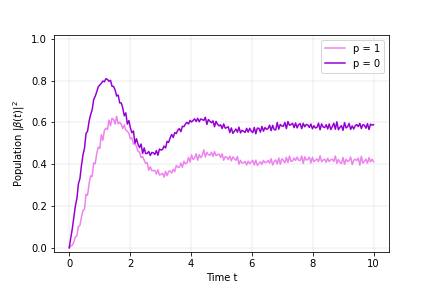
\includegraphics[width=\textwidth]{tex/figures/exercise07_02.png}
        \caption{Population $\abs{\beta}^2$ over time $t$ for $\gamma = 0.01$ and $p = 0.095$ and $0.05$. A lower $p$ corresponds to a higher thermal excitation rate and higher asymptote.}
        \label{fig:exercise07_02}
    \end{subfigure}
    \begin{subfigure}[t]{0.48\textwidth}
        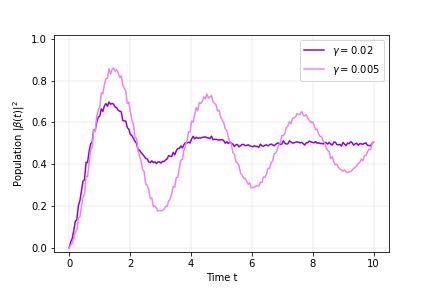
\includegraphics[width=\textwidth]{tex/figures/exercise07_03.png}
        \caption{Population $\abs{\beta}^2$ over time $t$ for $p = 0.5$ and $\gamma = 0.002$ and $0.005$. A higher $\gamma$ corresponds to a higher spontaneous emission rate and stronger dampening, which is clearly visible for $\gamma = 0.02$.}
        \label{fig:exercise07_03}
    \end{subfigure}
    \\
    \begin{subfigure}[b]{\textwidth}
        \centering
        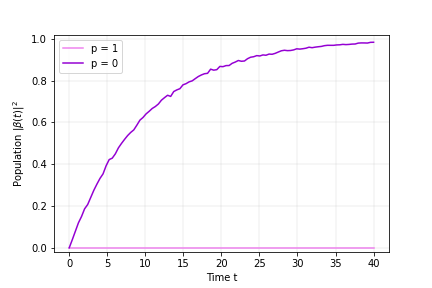
\includegraphics[width=0.48\textwidth]{tex/figures/exercise07_04.png}
        \caption{Population $\abs{\beta}^2$ over time $t$ for $\gamma = 0.02$ and $p = 1$ and $0$, without a driving term. At $p = 0$ GAD is an amplitude enhancing channel, that eventually turns all initial states to $\ket{1}$. With $p = 1$ GAD equals to the normal dampening channel, where all initial states end up in $\ket{0}$.}
        \label{fig:exercise07_04}
    \end{subfigure}
\end{figure}

\section{Single-Qubit Tomography}
Quantum state tomography is the method for reconstructing a qubit state by measuring the expectation values of the Pauli operators $\hat{\sigma}_i$. One can reconstruct the qubit state from these expectation values because the Pauli operators form an orthonormal basis of the $2\times2$ Hilbert space. Thus every qubit density matrix $\rho$ can be expressed as
\begin{equation}
    \rho = \Vec{c} \cdot \Vec{\hat{\sigma}}
\end{equation}
with $\Vec{\hat{\sigma}} = \{\mathbb{1}, \sigmax,\sigmay, \sigmaz\}$ the pseudo-vector of Pauli matrices and the vector coefficients  $\vec{c} = \frac{1}{2}\langle\Vec{\hat{\sigma}}\rangle$. Measuring the identity matrix contribution is not necessary since it's defined by the normalization condition $\operatorname{Tr}(\rho) =1 \rightarrow c_0 = \frac{1}{2}$. 

Usually the measurement basis for a quantum system is the z-basis. To measure $\langle\sigmax\rangle$ and $\langle\sigmay\rangle$ we need to perform a basis transformation from the measurement basis to the desired one using the cirq native gate set.
\subsubsection{Exercise 8}
The basis transformations for measurements in the x- and y-basis are
\begin{equation}
\yx{HZH} = \frac{1}{\sqrt{2}}\begin{pmatrix} 1&1\\1&1\end{pmatrix} \begin{pmatrix} 1&0\\0&-1\end{pmatrix}  \frac{1}{\sqrt{2}}\begin{pmatrix} 1&1\\1&1\end{pmatrix}  = \begin{pmatrix} 0&1\\1&0\end{pmatrix} = \yx{X} ,
\end{equation}
\begin{equation}
    \yx{SHZHS^\dagger} = \begin{pmatrix} 1&0\\0&i\end{pmatrix}\hadamard \begin{pmatrix} 1&0\\0&-1\end{pmatrix} \hadamard \begin{pmatrix} 1&0\\0&-i\end{pmatrix} = \begin{pmatrix} 0&-i\\i&0\end{pmatrix} = \yx{Y}.
\end{equation}
We demonstrate the quantum state tomography using cirq by simulating the measurement of the coefficient vector $\vec{c}$ and reconstructing the density matrix for the state $\ket{\Psi} = TH\ket{0} = \frac{1}{\sqrt{2}} \left(\ket{0} + e^{i\frac{\pi}{4}}\ket{1}\right)$. The measurements yield 
\begin{equation}
\vec{c} = \frac{1}{2}\begin{pmatrix}1\\0.000976\\0.706706\\0.706706\end{pmatrix}
\end{equation}
for the coefficients and thus for the reconstructed density matrix:
\begin{equation}
    \rho = \begin{pmatrix}0.500488 & 0.353353-0.353353\iu \\0.353353+0.353353\iu & 0.499512\end{pmatrix}
\end{equation}
To extract the qubit state from this density we must simply remind ourselves that an arbitrary desinty matrix for a pure qubit state is given by 

\begin{equation}
\rho = \begin{pmatrix} \abs{\alpha^2}& \alpha\beta^*\\\alpha^*\beta& \abs{\beta^2} \end{pmatrix}.
\end{equation}
We can therefore simply read-off the qubit state to be: $\ket{\Psi}_{tomo} = 0.70745196 \ket{0} + (0.4997558 +0.4997558\iu) \ket{1}$. We can thus see that the single-qubit tomography method reconstructs $\ket{\Psi}$ very well.

Equipped with this knowledge, we can now confidently use this method to reconstruct the oscillating qubit state from the Rabi oscillation. Figure \ref{fig:tomo} shows the population of the $\ket{1}$ state calculated using the analytical solution from equation \eqref{eq:population1} and using single-qubit tomography. As expected, the tomography reconstruction agrees well with the analytical solution.

\begin{figure}[h]
    \centering
    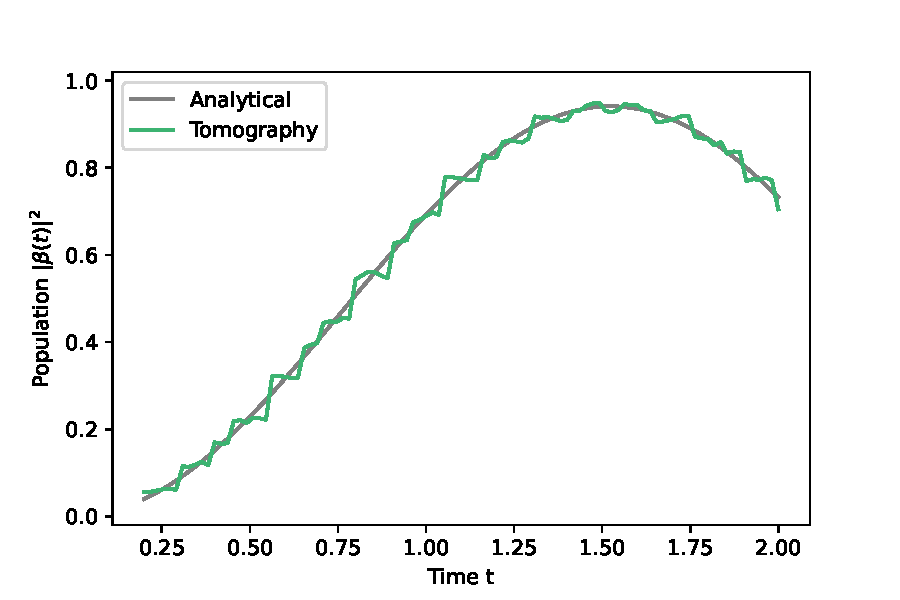
\includegraphics[width = 0.7\textwidth]{tex/figures/exercise10.pdf}
    \caption{Population $\abs{\beta}^2$ over time $t$ during a Rabi oscillation. State calculated using the analytical equation \eqref{eq:population1} and the state tomography sequence.}
    \label{fig:tomo}
\end{figure}

\section{Variational Quantum Eigensolver}
The variational quantum eigensolver (VQE) is a hybrid
quantum-classical algorithm that makes use of the variational method to find eigenvalues of a Hamiltonian. Let us consider a two-qubit cluster state Hamiltonian:
\begin{equation}
    \hat{H} = -\sigmax^1\sigmaz^2 - \sigmaz^1\sigmax^2
    \label{eq:HamVQE}
\end{equation} There are two main steps to applying the VQE algorithm. 

First, we construct a parameterized circuit ansatz, as seen in figure \ref{fig:variational_ansatz} which prepares the trial state: 
\begin{equation}
    \label{eq:trialstate}
    \ket{\psi(a, b)} = \exp\left[\mathrm{i}a \left(\sigmaz^1+\sigmaz^2\right)\right] \exp\left[\mathrm{i}b\left(\sigmax^1\sigmaz^2 + \sigmaz^1\sigmax^2\right)\right] \ket{00}
\end{equation}
To do so we define the two two-qubit gates $\mathrm{RZX} = \exp\left(\mathrm{i}b\left(\sigmaz \otimes \sigmax\right)\right)$ and $\mathrm{RXZ} = \exp\left(\mathrm{i}b\left(\sigmax \otimes \sigmaz\right)\right)$. 

\begin{figure}[h]
    \centering
    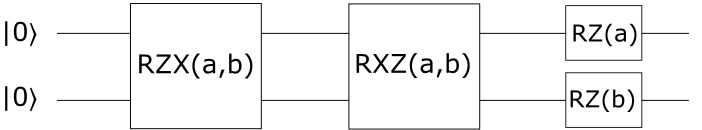
\includegraphics[width=0.6\linewidth]{tex/figures/CircuitEx10.png}
    \caption{Quantum circuit for creating the parameterized trial state from equation \eqref{eq:trialstate}}
    \label{fig:variational_ansatz}
\end{figure}

To find the minimum energy state, we make use of a simple grid search over the whole parameter space for a and b. For each choice a and b, we measure the energy expectation value and plot the results on a heat map to find the best trial state. 

\begin{figure}[h]
    \centering
    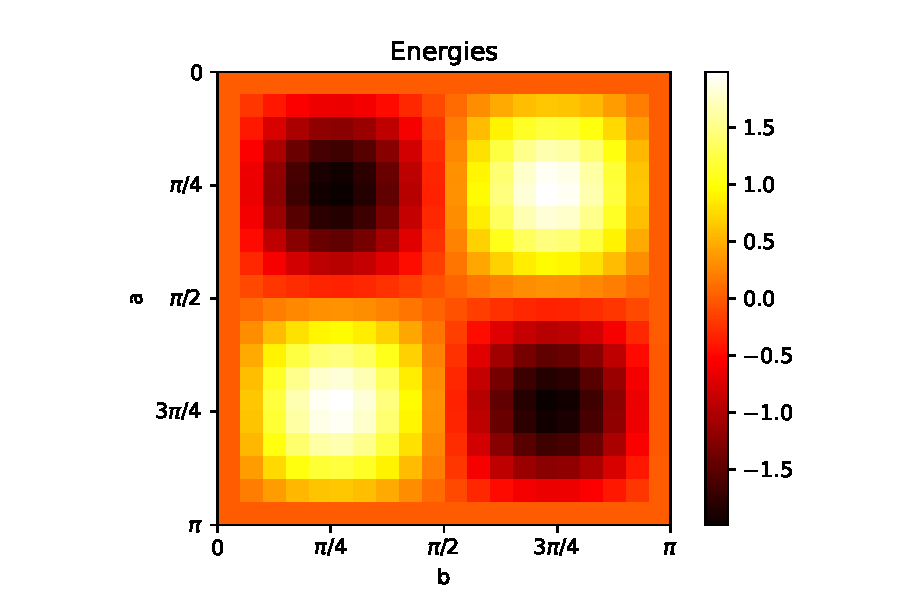
\includegraphics[width=0.8\linewidth]{tex/figures/exercise12.pdf}
    \caption{Energy expectation value for the Hamiltonian \eqref{eq:HamVQE} as a function of the trial state parameters a and b defined in \eqref{eq:trialstate}.}
    \label{fig:heatmap1}
\end{figure}

Using the best trial state, we find an approximate ground state energy of $E_0 = -1.986$.

To benchmark the approximate solution, we compare it to the exact solution of the ground state:
\begin{equation}
    \ket{\mathrm{\psi}} = \frac{1}{\sqrt{2}} \left(\ket{1-} + \ket{0+} \right)
\end{equation}
\begin{equation}
    \hat{H}\ket{\psi} = \left(-\sigmax^1\sigmaz^2 - \sigmaz^1\sigmax^2 \right) \left(\frac{1}{\sqrt{2}} \left(\ket{1-} + \ket{0+} \right)\right) = -2\ket{\psi}
\end{equation}

So we see that the approximation agrees well with the exact solution of $E_0 = -2$.

Lastly, we compute a landscape for the bipartition entanglement entropy over the parameter grid, see heat map \ref{fig:Ex15}, and compare it to the energy landscape. The first thing one notes is that, unlike the energy landscape, the entanglement entropy is independent of $a$ (within numerical accuracy). This is to be expected, since the rotations that depend on $a$ are local unitaries which cannot influence entanglement. The second thing one notices is that areas with high absolute energy value correspond to areas of high entanglement entropy except when $a\approx\frac{\pi}{2}$, in which case $a$ introduces a relative phase between the terms such that the energy vanishes.
\begin{figure}
    \centering
    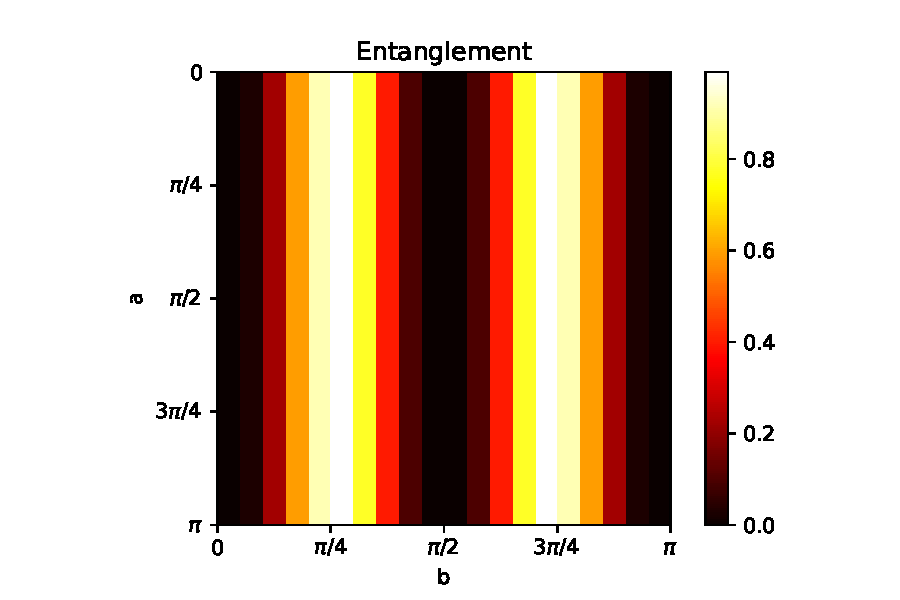
\includegraphics[width = 0.8\textwidth]{tex/figures/exercise15.pdf}
    \caption{Bipartition entanglement entropy of the trial state from equation \eqref{eq:trialstate} as a function of the parameters $a$ and $b$.}
    \label{fig:Ex15}
\end{figure}